\chapter{Relacions Trigonom\`{e}triques}\index{trigonometria}

\section{Funcions Trigonom\`{e}triques}\index{funcions trigonom\`{e}triques}

En la Taula \vref{taula:func-trig-signes} es pot veure el signe de
les funcions trigonom\`{e}triques, segons en quin dels quatre quadrants
es trobi l'angle $\alpha$. I: $\alpha\in[0,\frac{\piup}{2}]$, II:
$\alpha\in[\frac{\piup}{2},\piup]$, III:
$\alpha\in[\piup,\frac{3\piup}{2}]$, IV:
$\alpha\in[\frac{3\piup}{2},2\piup]$.
\index{sin}\index{cos}\index{tan}\index{csc}\index{sec}\index{cot}

\begin{table}[h]
   \caption{\label{taula:func-trig-signes} Signes de les funcions trigonom\`{e}triques ens el quatre quadrants}
   \begin{center}\begin{tabular}{cccc|cccc}
   $\sin\alpha > 0$ & $\cos\alpha < 0$ & $\tan\alpha < 0$ & & &
   $\sin\alpha > 0$ & $\cos\alpha > 0$ & $\tan\alpha > 0$ \\
   $\csc\alpha > 0$ & $\sec\alpha < 0$ & $\cot\alpha < 0$ & \textbf{II}&
   \textbf{I} & $\csc\alpha > 0$ & $\sec\alpha > 0$ & $\cot\alpha > 0$ \\
   \hline
   $\sin\alpha < 0$ & $\cos\alpha < 0$ & $\tan\alpha > 0$
   &\textbf{III} &
   \textbf{IV} & $\sin\alpha < 0$ & $\cos\alpha > 0$ & $\tan\alpha < 0$ \\
   $\csc\alpha < 0$ & $\sec\alpha < 0$ & $\cot\alpha > 0$  & & &
   $\csc\alpha < 0$ & $\sec\alpha > 0$ & $\cot\alpha < 0$
   \end{tabular} \end{center}
\end{table}


 Es presenten a continuaci\'{o}  les funcions trigonom\`{e}triques d'angles en qualsevol
quadrant, en funci\'{o} d'un angle en el primer quadrant,
$\alpha\in[0,\frac{\piup}{2}]$.
\begin{subequations}
\begin{align}
    \sin(-\alpha) &= -\sin\alpha  & \csc(-\alpha) &= -\csc\alpha \\
    \cos(-\alpha) &= +\cos\alpha  & \sec(-\alpha) &= +\sec\alpha \\
    \tan(-\alpha) &= -\tan\alpha  & \cot(-\alpha) &= -\cot\alpha
\end{align}
\end{subequations}
\vspace{-5mm}
\begin{subequations}
\begin{align}
    \sin\left(\frac{\piup}{2}\pm\alpha\right) &= +\cos\alpha    & \csc\left(\frac{\piup}{2}\pm\alpha\right) &= +\sec\alpha \\
    \cos\left(\frac{\piup}{2}\pm\alpha\right) &= \mp\sin\alpha  & \sec\left(\frac{\piup}{2}\pm\alpha\right) &= \mp\csc\alpha \\
    \tan\left(\frac{\piup}{2}\pm\alpha\right) &= \mp\cot\alpha  & \cot\left(\frac{\piup}{2}\pm\alpha\right) &= \mp\tan\alpha
\end{align}
\end{subequations}
\vspace{-5mm}
\begin{subequations}
\begin{align}
    \sin(\piup\pm\alpha) &= \mp\sin\alpha  & \csc(\piup\pm\alpha) &= \mp\csc\alpha \\
    \cos(\piup\pm\alpha) &= -\cos\alpha    & \sec(\piup\pm\alpha) &= -\sec\alpha \\
    \tan(\piup\pm\alpha) &= \pm\tan\alpha  & \cot(\piup\pm\alpha) &= \pm\cot\alpha
\end{align}
\end{subequations}
\vspace{-5mm}
\begin{subequations}
\begin{align}
    \sin\left(\frac{3\piup}{2}\pm\alpha\right) &= -\cos\alpha    & \csc\left(\frac{3\piup}{2}\pm\alpha\right) &= -\sec\alpha \\
    \cos\left(\frac{3\piup}{2}\pm\alpha\right) &= \pm\sin\alpha  & \sec\left(\frac{3\piup}{2}\pm\alpha\right) &= \pm\csc\alpha \\
    \tan\left(\frac{3\piup}{2}\pm\alpha\right) &= \mp\cot\alpha  & \cot\left(\frac{3\piup}{2}\pm\alpha\right) &= \mp\tan\alpha
\end{align}
\end{subequations}
\vspace{-5mm}
\begin{subequations}
\begin{align}
    \sin(2\piup\pm\alpha) &= \pm\sin\alpha  & \csc(2\piup\pm\alpha) &= \pm\csc\alpha \\
    \cos(2\piup\pm\alpha) &= +\cos\alpha    & \sec(2\piup\pm\alpha) &= +\sec\alpha \\
    \tan(2\piup\pm\alpha) &= \pm\tan\alpha  & \cot(2\piup\pm\alpha) &= \pm\cot\alpha
\end{align}
\end{subequations}

En la Taula \vref{taula:func-trig-angles} es pot veure el valor de
les funcions trigonom\`{e}triques per a diversos angles usuals.
\begin{table}[h]
   \caption{\label{taula:func-trig-angles} Valors de les funcions trigonom\`{e}triques per a diversos angles}
   \begin{center}\begin{tabular}{cccccccc}
   \toprule[1pt]
    \multicolumn{2}{c}{$\alpha$} &
    \multirow{2}{15mm}{\hspace{2ex}\rule{0mm}{6mm}$\sin\alpha$} &
    \multirow{2}{15mm}{\hspace{2ex}\rule{0mm}{6mm}$\cos\alpha$}  &
    \multirow{2}{15mm}{\hspace{2ex}\rule{0mm}{6mm}$\tan\alpha$} &
    \multirow{2}{15mm}{\hspace{2ex}\rule{0mm}{6mm}$\csc\alpha$} &
    \multirow{2}{15mm}{\hspace{2ex}\rule{0mm}{6mm}$\sec\alpha$}  &
    \multirow{2}{15mm}{\hspace{2ex}\rule{0mm}{6mm}$\cot\alpha$}\\
    \cmidrule(rl){1-2}
    [rad] & [\degree] & & & & & & \\
   \midrule
   0 & 0 & 0 & 1 & 0 & $\pm\infty$ & 1 & $\pm\infty$\\[1ex]
   $\dfrac{\piup}{6}$ & 30 & $\dfrac{1}{2}$ & $\dfrac{\sqrt{3}}{2}$ &
   $\dfrac{\sqrt{3}}{3}$ & 2 & $\dfrac{2\sqrt{3}}{3}$ & $\sqrt{3}$\\[1.5ex]
   $\dfrac{\piup}{4}$ & 45 & $\dfrac{\sqrt{2}}{2}$  &
   $\dfrac{\sqrt{2}}{2}$ & 1 & $\sqrt{2}$ & $\sqrt{2}$ & 1\\[1.5ex]
   $\dfrac{\piup}{3}$ & 60 &  $\dfrac{\sqrt{3}}{2}$ & $\dfrac{1}{2}$ &
   $\sqrt{3}$ & $\dfrac{2\sqrt{3}}{3}$ & 2 & $\dfrac{\sqrt{3}}{3}$\\[2ex]
   $\dfrac{\piup}{2}$ & 90 & 1 & 0 & $\pm\infty$ & 1 & $\pm\infty$ & 0\\[1.5ex]
   $\piup$ & 180 & 0 & $-1$ & 0 & $\pm\infty$ & $-1$ & $\pm\infty$\\[1ex]
   $\dfrac{3\piup}{2}$ & 270 & $-1$ & 0 & $\pm\infty$ & $-1$ & $\pm\infty$ & 0\\
   \bottomrule[1pt]
   \end{tabular} \end{center}
\end{table}

Es d\'{o}na a continuaci\'{o} cadascuna de les funcions trigonom\`{e}triques, en
funci\'{o} de totes les altres. Els signe $\pm$ que apareix en les
equacions, ve determinat pel quadrant on es troba l'angle $\alpha$
(vegeu la Taula \vref{taula:func-trig-signes}).
\begin{subequations}
\begin{align}
\sin\alpha &= \pm\sqrt{1-\cos^2\alpha} =
\frac{\tan\alpha}{\pm\sqrt{1+\tan^2\alpha}} =
\frac{1}{\pm\sqrt{1+\cot^2\alpha}} =
\frac{\pm\sqrt{\sec^2\alpha-1}}{\sec\alpha} = \frac{1}{\csc\alpha}\\[1.6ex]
\cos\alpha &= \pm\sqrt{1-\sin^2\alpha} =
\frac{1}{\pm\sqrt{1+\tan^2\alpha}} =
\frac{\cot\alpha}{\pm\sqrt{1+\cot^2\alpha}} = \frac{1}{\sec\alpha} =
\frac{\pm\sqrt{\csc^2\alpha-1}}{\csc\alpha}\\[1.6ex]
\tan\alpha &= \frac{\sin\alpha}{\pm\sqrt{1-\sin^2\alpha}} =
\frac{\pm\sqrt{1-\cos^2\alpha}}{\cos\alpha} = \frac{1}{\cot\alpha} =
\pm\sqrt{\sec^2\alpha-1} =
 \frac{1}{\pm\sqrt{\csc^2\alpha-1}}\displaybreak\\[1.6ex]
\csc\alpha &= \frac{1}{\sin\alpha} =
\frac{1}{\pm\sqrt{1-\cos^2\alpha}} =
\frac{\pm\sqrt{1+\tan^2\alpha}}{\tan\alpha} =
\pm\sqrt{1+\cot^2\alpha} =
\frac{\sec\alpha}{\pm\sqrt{\sec^2\alpha-1}}\\[1.6ex]
\sec\alpha &= \frac{1}{\pm\sqrt{1-\sin^2\alpha}} =
\frac{1}{\cos\alpha} = \pm\sqrt{1+\tan^2\alpha} =
\frac{\pm\sqrt{1+\cot^2\alpha}}{\cot\alpha} =
\frac{\csc\alpha}{\pm\sqrt{\csc^2\alpha-1}}\\[1.6ex]
\cot\alpha &= \frac{\pm\sqrt{1-\sin^2\alpha}}{\sin\alpha} =
\frac{\cos\alpha}{\pm\sqrt{1-\cos^2\alpha}} = \frac{1}{\tan\alpha} =
\frac{1}{\pm\sqrt{\sec^2\alpha-1}} = \pm\sqrt{\csc^2\alpha-1}
\end{align}
\end{subequations}

Identitats fonamentals de les funcions trigonom\`{e}triques:
\begin{gather}
    \sin^2\alpha + \cos^2\alpha = 1 \\
    1 + \tan^2\alpha = \sec^2\alpha\\
    1 + \cot^2\alpha = \csc^2\alpha\\
    \cos\alpha + \ju \sin\alpha = \eu^{\ju\alpha}
\end{gather}

Funcions trigonom\`{e}triques de l'angle doble, i generalitzaci\'{o} per a
$n\in\mathbb{Z}$:
\begin{subequations}
\begin{align}
    \sin 2\alpha &= 2 \sin\alpha \cos\alpha & \sin n \alpha &=
    2\sin[(n-1)\alpha]\cos \alpha -\sin[(n-2)\alpha]\\[1ex]
    \cos 2\alpha &= 2\cos^2\alpha -1 & \cos n\alpha &=
    2\cos[(n-1)\alpha]\cos \alpha -\cos[(n-2)\alpha]\\[1ex]
    \tan 2\alpha &=\frac{2\tan\alpha}{1-\tan^2\alpha} & \tan n
    \alpha &= \frac{\tan[(n-1)\alpha]+\tan\alpha}{1-\tan[(n-1)\alpha]\tan\alpha}
\end{align}
\end{subequations}


Funcions trigonom\`{e}triques de l'angle meitat. Els signe $\pm$ que
apareix en les equacions, ve determinat pel quadrant on es troba
l'angle $\frac{\alpha}{2}$ (vegeu la Taula
\vref{taula:func-trig-signes}):
\begin{subequations}
\begin{align}
    \sin \frac{\alpha}{2} &= \pm \sqrt{\frac{1-\cos\alpha}{2}}\\[1ex]
    \cos \frac{\alpha}{2} &= \pm \sqrt{\frac{1+\cos\alpha}{2}}\\[1ex]
    \tan \frac{\alpha}{2} &= \pm \sqrt{\frac{1-\cos\alpha}{1+\cos\alpha}}
\end{align}
\end{subequations}


Funcions trigonom\`{e}triques de la suma i difer\`{e}ncia d'angles:
\begin{subequations}
\begin{align}
    \sin(\alpha+\beta) &= \sin\alpha \cos\beta + \sin\beta\cos\alpha &
    \sin(\alpha-\beta) &= \sin\alpha \cos\beta - \sin\beta\cos\alpha\\[1ex]
    \cos(\alpha+\beta) &= \cos\alpha \cos\beta - \sin\beta\sin\alpha &
    \cos(\alpha-\beta) &= \cos\alpha \cos\beta + \sin\beta\sin\alpha\\[1ex]
    \tan(\alpha+\beta) &=\frac{\tan\alpha+\tan\beta}{1-\tan\alpha\tan\beta} &
    \tan(\alpha-\beta)
    &=\frac{\tan\alpha-\tan\beta}{1+\tan\alpha\tan\beta}
\end{align}
\end{subequations}

Suma i difer\`{e}ncia de funcions trigonom\`{e}triques:
\begin{subequations}
\begin{align}
    \sin\alpha+\sin\beta &= 2 \sin\left(\frac{\alpha+\beta}{2}\right)
    \cos\left(\frac{\alpha-\beta}{2}\right)\\[1ex]
    \sin\alpha-\sin\beta &= 2 \cos\left(\frac{\alpha+\beta}{2}\right)
    \sin\left(\frac{\alpha-\beta}{2}\right)\\[1ex]
    \cos\alpha+\cos\beta &= 2 \cos\left(\frac{\alpha+\beta}{2}\right)
    \cos\left(\frac{\alpha-\beta}{2}\right)\\[1ex]
    \cos\alpha-\cos\beta &= -2 \sin\left(\frac{\alpha+\beta}{2}\right)
    \sin\left(\frac{\alpha-\beta}{2}\right)
\end{align}
\end{subequations}

Producte de funcions trigonom\`{e}triques:
\begin{subequations}
\begin{align}
    \sin\alpha \cos\beta &=
    \frac{\sin(\alpha-\beta)+\sin(\alpha+\beta)}{2}\\[1ex]
    \cos\alpha \cos\beta &=
    \frac{\cos(\alpha-\beta)+\cos(\alpha+\beta)}{2}\\[1ex]
    \sin\alpha \sin\beta &=
    \frac{\cos(\alpha-\beta)-\cos(\alpha+\beta)}{2}
\end{align}
\end{subequations}

Producte de funcions trigonom\`{e}triques del la suma i difer\`{e}ncia
d'angles:
\begin{subequations}
\begin{align}
    \sin(\alpha+\beta) \sin(\alpha-\beta) &= \sin^2\alpha-\sin^2\beta =
    \cos^2\beta - \cos^2\alpha\\[1ex]
    \cos(\alpha+\beta) \cos(\alpha-\beta) &= \cos^2\alpha-\sin^2\beta =
    \cos^2\beta - \sin^2\alpha
\end{align}
\end{subequations}

Pot\`{e}ncies de funcions trigonom\`{e}triques:
\begin{subequations}
\begin{align}
    \sin^2\alpha &= \frac{1-\cos 2\alpha}{2} &  \cos^2\alpha &= \frac{1+\cos 2\alpha}{2}\\[1ex]
    \sin^3\alpha &= \frac{3\sin\alpha-\sin 3\alpha}{4} &  \cos^3\alpha &= \frac{3\cos\alpha+\cos 3\alpha}{4}\\[1ex]
    \sin^4\alpha &= \frac{3-4\cos 2\alpha+\cos 4\alpha}{8} &  \cos^4\alpha &= \frac{3+4\cos 2\alpha+\cos 4\alpha}{8}
\end{align}
\end{subequations}

Conversi\'{o} de la suma d'una funci\'{o} cosinus i una funci\'{o} sinus, en una \'{u}nica
funci\'{o} cosinus\footnote{La funci\'{o} \textsf{arctan} torna de forma estandarditzada valors compresos entre $-\frac{\piup}{2}$ i $\frac{\piup}{2}$, \'{e}s per aix\`{o} que cal sumar el valor $\piup$ quan $A$ \'{e}s negatiu, per tal d'obtenir l'angle en el quadrant correcte.} ($A,B\in\mathbb{R}$):
\begin{align}
    A \cos \alpha + B \sin \alpha &= \begin{cases} \sqrt{A^2+B^2}\, \cos \left(\alpha - \arctan\dfrac{B}{A}\right), & A >0 \\[2ex]
    \sqrt{A^2+B^2}\, \cos \left(\alpha - \arctan\dfrac{B}{A}+\piup\right), & A<0 \end{cases}\label{eq:AcosBsin}
\end{align}

Conversi\'{o} de la suma d'una funci\'{o} cosinus i una funci\'{o} sinus, en una \'{u}nica
funci\'{o} sinus\footnotemark[1] ($A,B\in\mathbb{R}$):
\begin{align}
    A \cos \alpha + B \sin \alpha &= \begin{cases} \sqrt{A^2+B^2}\, \sin \left(\alpha - \arctan\dfrac{B}{A}+\dfrac{\piup}{2}\right), & A >0 \\[2ex]
    \sqrt{A^2+B^2}\, \sin \left(\alpha - \arctan\dfrac{B}{A}+\dfrac{3\piup}{2}\right), & A<0 \end{cases}\label{eq:AcosBsinS}
\end{align}

\section{Lleis dels sinus, cosinus i tangents}\label{sec:llei-s-c-t}

Les lleis del sinus, cosinus i tangents, relacionen les longituds
dels tres costats $a$, $b$ i $c$ d'un triangle qualsevol, com el de
la Figura \vref{pic:llei-s-c-t}, amb els seus tres angles interiors
$\alpha$, $\beta$ i $\gamma$, i amb el radi $R$ de la circumfer\`{e}ncia circumscrita al triangle.

\begin{figure}[htb]
\centering
    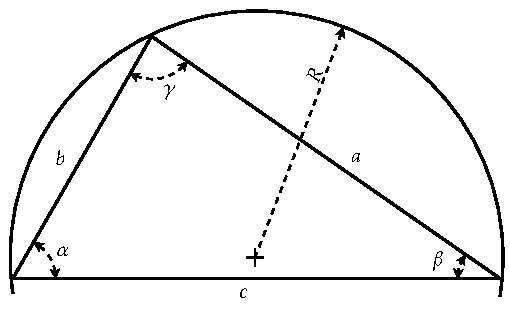
\includegraphics{Imatges/Ape-Trigonometria-Triangle.pdf}
\caption{Lleis dels sinus, cosinus i tangents} \label{pic:llei-s-c-t}
\end{figure}

La llei dels sinus ens d\'{o}na la relaci\'{o} seg\"{u}ent:\index{llei dels
sinus}
\begin{equation}
    \frac{a}{\sin\alpha} = \frac{b}{\sin\beta} =
    \frac{c}{\sin\gamma} = 2 R
\end{equation}

La llei dels cosinus ens d\'{o}na les relacions seg\"{u}ents:\index{llei
dels cosinus}
\begin{subequations}
\begin{align}
    a^2 &= b^2 + c^2 - 2 b c \cos\alpha \\[1ex]
    b^2 &= a^2 + c^2 - 2 a c \cos\beta \\[1ex]
    c^2 &= a^2 + b^2 - 2 a b \cos\gamma
\end{align}
\end{subequations}

La llei de les tangents ens d\'{o}na les relacions seg\"{u}ents:\index{llei
de les tangents}
\begin{subequations}
\begin{align}
    \frac{a-b}{a+b} &= \frac{\tan\frac{\alpha-\beta}{2}}{\tan\frac{\alpha+\beta}{2}} \\[1ex]
    \frac{a-c}{a+c} &= \frac{\tan\frac{\alpha-\gamma}{2}}{\tan\frac{\alpha+\gamma}{2}} \\[1ex]
    \frac{b-c}{b+c} &= \frac{\tan\frac{\beta-\gamma}{2}}{\tan\frac{\beta+\gamma}{2}}
\end{align}
\end{subequations}

\section{Funcions Hiperb\`{o}liques}\index{funcions hiperb\`{o}liques}

Definici\'{o} de les funcions hiperb\`{o}liques ($z\in\mathbb{C}$):
\begin{subequations}
\begin{align}
    \sinh z&\equiv \frac{\eu^z - \eu^{-z}}{2} & \csch z &\equiv\frac{1}{\sinh z} =
    \frac{2}{\eu^z - \eu^{-z}}\\[1ex]
    \cosh z&\equiv \frac{\eu^z + \eu^{-z}}{2} & \sech z &\equiv\frac{1}{\cosh z} =
    \frac{2}{\eu^z + \eu^{-z}}\\[1ex]
    \tanh z&\equiv \frac{\sinh z}{\cosh z} = \frac{\eu^{2z}-1}{\eu^{2z}+1} &
    \coth z &\equiv\frac{1}{\tanh z} = \frac{\eu^{2z}+1}{\eu^{2z}-1}
\end{align}
\end{subequations}
\index{sinh}\index{cosh}\index{tanh}\index{csch}\index{sech}\index{coth}

Identitats fonamentals de les funcions hiperb\`{o}liques
($z\in\mathbb{C}$):
\begin{align}
    &\cosh^2 z - \sinh^2 z = 1 \\
    &\sech^2 z + \tanh^2 z = 1 \\
    &\csch^2 z - \coth^2 z = -1 \\
    &\cosh z + \sinh z = \eu^z
\end{align}

Les funcions hiperb\`{o}liques presenten les seg\"{u}ents simetries
($z\in\mathbb{C}$):
\begin{subequations}
\begin{align}
    \sinh (-z) &= -\sinh z \\
    \cosh (-z) &= \cosh z\\
    \tanh (-z) &= -\tanh z
\end{align}
\end{subequations}

Funcions hiperb\`{o}liques de la suma i difer\`{e}ncia d'arguments ($z_1,
z_2\in\mathbb{C}$):
\begin{subequations}
\begin{align}
    \sinh(z_1+z_2) &= \sinh z_1 \cosh z_2 + \sinh z_2\cosh z_1\\[1ex]
    \sinh(z_1-z_2) &= \sinh z_1 \cosh z_2 - \sinh z_2\cosh z_1\\[1ex]
    \cosh(z_1+z_2) &= \cosh z_1 \cosh z_2 + \sinh z_2\sinh z_1\\[1ex]
    \cosh(z_1-z_2) &= \cosh z_1 \cosh z_2 - \sinh z_2\sinh z_1\\[1ex]
    \tanh(z_1+z_2) &=\frac{\tanh z_1+\tanh z_2}{1+\tanh z_1\tanh z_2}\\[1ex]
    \tanh(z_1-z_2) &=\frac{\tanh z_1-\tanh z_2}{1-\tanh z_1\tanh z_2}
\end{align}
\end{subequations}

Suma i difer\`{e}ncia de funcions hiperb\`{o}liques ($z_1,
z_2\in\mathbb{C}$):
\begin{subequations}
\begin{align}
    \sinh z_1+\sinh z_2 &= 2 \sinh\left(\frac{z_1+z_2}{2}\right)
    \cosh\left(\frac{z_1-z_2}{2}\right)\\[1ex]
    \sinh z_1-\sinh z_2 &= 2 \cosh\left(\frac{z_1+z_2}{2}\right)
    \sinh\left(\frac{z_1-z_2}{2}\right)\\[1ex]
    \cosh z_1+\cosh z_2 &= 2 \cosh\left(\frac{z_1+z_2}{2}\right)
    \cosh\left(\frac{z_1-z_2}{2}\right)\\[1ex]
    \cosh z_1-\cosh z_2 &= 2 \sinh\left(\frac{z_1+z_2}{2}\right)
    \sinh\left(\frac{z_1-z_2}{2}\right)
\end{align}
\end{subequations}

Producte de funcions hiperb\`{o}liques ($z_1, z_2\in\mathbb{C}$):
\begin{subequations}
\begin{align}
    \sinh z_1 \cosh z_2 &=
    \frac{\sinh(z_1+z_2)+\sinh(z_1-z_2)}{2}\\[1ex]
    \cosh z_1 \cosh z_2 &=
    \frac{\cosh(z_1+z_2)+\cosh(z_1-z_2)}{2}\\[1ex]
    \sinh z_1 \sinh z_2 &=
    \frac{\cosh(z_1+z_2)-\cosh(z_1-z_2)}{2}
\end{align}
\end{subequations}
